\documentclass{article}
\usepackage[utf8]{inputenc}
\usepackage{graphicx}
\usepackage{listings}
\usepackage{booktabs}

\title{Lab 3}
\author{Hannah Atmer \and Xiaoyue Chen \\ Team 6}
\date{October 2021}

\begin{document}

\maketitle
\section{Hardware}
\subsection{CPU}
\begin{verbatim}
Architecture              x86_64
CPU(s)                    12
Model name                Intel(R) Core(TM) i7-8750H CPU
Thread(s) per core        2
Core(s) per socket        6
CPU max MHz               4100.0000
\end{verbatim}

\subsection{GPU}
\begin{verbatim}
Device Name               NVIDIA GeForce GTX 1060
PCIe Version              3.0.0
Max compute units         10
Max clock frequency       1733MHz
Cuda cores                1280
\end{verbatim}

\section{Performance Estimates}
For loading, we assume that we are reading from an huge array that
cannot fit into L3. See table \ref{tab:estcpu} and \ref{tab:estgpu}.

\begin{table}[h!]
  \centering
  \begin{tabular}{lll}
    \toprule
    Operation & Prediction & Why \\
    \midrule
    add char & 2361 GOPS & \(6~\mathit{cores} \times 4.1~\mathit{GHz} \times
                           32~\mathit{AVX} \times 3~\mathit{ports}\) \\
    add float & 590 GFLOPS & \(6~\mathit{cores} \times 4.1~\mathit{GHz} \times
                             8~\mathit{AVX} \times 3~\mathit{ports}\) \\
    load seq & 14.4 GB/S & benchmark \\
    load rand & 0.9 GOPS & \(14.4 \div 16\) (only using
                           \(\frac{4}{64}\) of cache line)\\
    \bottomrule
  \end{tabular}
  \caption{Performance estimation for CPU}
  \label{tab:estcpu}
\end{table}
  \begin{table}[h!]
    \centering
    \begin{tabular}{lll}
      \toprule
      Operation & Predicted & Why \\
      \midrule
      add char & 1632 GOPS & \(10~\mathit{SM} \times (64+32)~\mathit{cores}
                             \times 1.7~\mathit{GHz}\) \\
      add float & 1632 GFLOPS & \(10~\mathit{SM} \times
                                (64+32)~\mathit{cores} \times
                                1.7~\mathit{GHz}\) \\
      load seq & 192 GB/s & specification \\
      load rand & 6 GB/s & \(192 \div 32\) (only using
                           \(\frac{4}{128}\) of cache line) \\
      transfer data & 1.5 GB/s & measured previously \\
      \bottomrule
    \end{tabular}
    \caption{Performance estimation for GPU}
    \label{tab:estgpu}
  \end{table}

\section{The given benchmarks}
Our compiler is gcc (GCC) 11.1.0.

\subsection{Why were all benchmark runs not the same speed in 1 and
  2?}
Benchmark 1 never uses \verb|sum| after computing it while benchmark 2
prints it out. The compiler optimises away the computation of \verb|sum|
in benchmark 1.

\subsection{What was the problem with 1 and 2 that we fixed in 3?}
We got rid the load instruction in benchmark 3.

\subsection{What optimization did the compiler do for 1 that prevented
  us from measuring what we wanted?}
The compiler does not generate any assembly related to \verb|sum| because
it is never used elsewhere.

\subsection{What did the code change in 2 do to prevent the compiler
  from doing this optimization?}
Benchmark 2 prints the \verb|sum|. Now \verb|sum| causes side effects.

\subsection{What optimization did the compiler do for 3 that prevented
  us from measuring what we wanted?}
The compiler issues multiply instruction instead of the looping add.

\subsection{Why was the performance of 4 so much slower than 2?}
Benchmark 2 issues AVX instructions.

\subsection{What was the optimization in 6 and why does it improve
  performance?}
In theory, benchmark 6 will have 3x performance of benchmark 5 because
our cpu have 3 ports on each core that can execute vector instructions
at the same cycle. However, it is not the case in reality. The
compiler figured out the same thing in benchmark 5 and unwrapped the
loop automatically for us. So we do not see any difference in
performance.

% Results
\section{Performance Achieved}

\subsection{Your measured performance results}
\begin{table}[h!]
  \centering
  \begin{tabular}{lllll}
    \toprule
    Operation & Predicted CPU &  Predicted GPU & Measured CPU & Measured GPU \\
    \midrule
    add char & 2361 GOPS & 1632 GOPS & 730 GOPS & 1390 GOPS \\
    add float & 590 GFLOPS & 1632 GFLOPS & 90 GFLOPS & 1597 GFLOPS \\
    load seq & 14.4 GB/s & 192 GB/s & 6.1 GB/s & 3.3 GB/s \\
    load rand & 0.9 GB/s & 1.5 GB/s & 0.05 GB/s & 0.023 GB/s \\
    transfer data & N/A & 1.5 GB/s & N/A & 4.1 GB/s \\
    \bottomrule
  \end{tabular}
  \caption{Prediction and measured results}
  \label{tab:pnm}
\end{table}

\subsection{Graph of results}

\begin{figure}[h!t]
  \centering 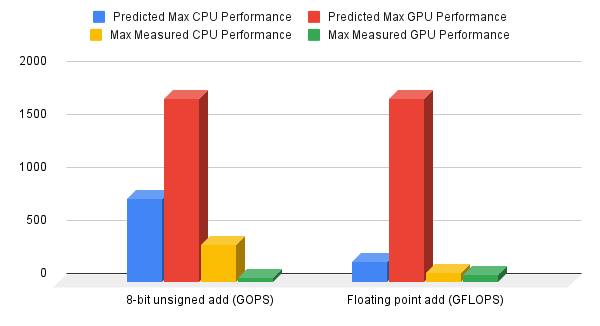
\includegraphics[width=1\textwidth]{add.png}
  \caption{Actual Performance Impact: Adding}
  \label{fig:add}
\end{figure}

\begin{figure}[h!t]
  \centering 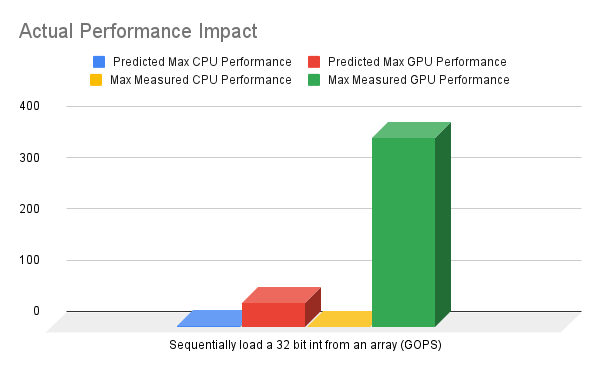
\includegraphics[width=1\textwidth]{sequential.png}
  \caption{Actual Performance Impact: Sequential Load}
  \label{fig:sequential}
\end{figure}

\begin{figure}[h!t]
  \centering 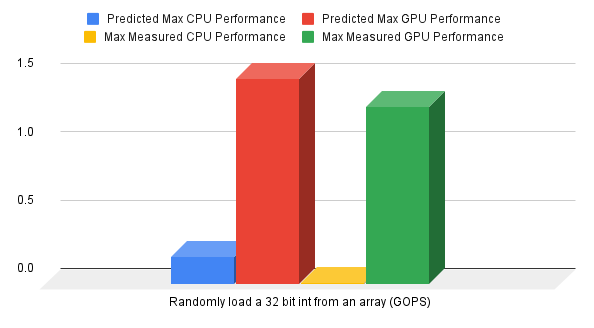
\includegraphics[width=1\textwidth]{random.png}
  \caption{Actual Performance Impact: Random Load}
  \label{fig:random}
\end{figure}

\begin{figure}[h!t]
  \centering 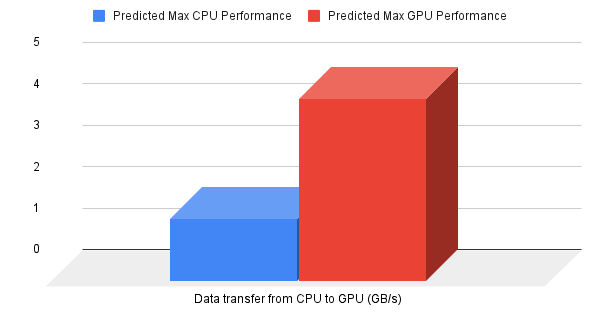
\includegraphics[width=1\textwidth]{dataTransfer.png}
  \caption{Actual Performance Impact: Data Transfer}
  \label{fig:transfer}
\end{figure}

% Discussion
\section{Discussion}

\subsection{A discussion of the measured results and how they differ
  from your predictions.}
Measured CPU performance is generally much worse than our predictions.
The arithmetic performance of the GPU is quite close to the
predictions.

It is also worth noting that the memory (load) performance are
generally much worse than the expectations. This is especially evident
when loading random elements in a big array.

\subsection{A discussion of what you learned about the hardware from
  measuring its performance.}
CPUs are usually quite busy because they need to multi-programme.
Hence it is difficult to get close to theoretical peak performance of
CPUs. On the other hand, GPUs seem to be less busy and we could get
close to their peak performance.

Another interesting fact is that memory performance seems to depend on
multi-threading. We could not get close to the theoretical peak memory
performance with loads from a single core.

Not being able to utilise the cache-lines (in the case of random
loading) means great losses to performance.

\subsection{A discussion of how you wrote your benchmarks and any
  issues you encountered and how you solved them.}
There are multiple ways to control the CPU benchmarks: compiler flags,
attributes, intrinsics, and inline assembly. We could also check the
generated assembly. Combining these methods, writing benchmarks for
CPU would become reasonably easy and clear.

However, it is the opposite for writing GPU benchmarks. OpenCL does
not output any assembly. It is hard to know what the compiler does. We
had to run the same benchmark with different values to observe the
changes in output to guess if the benchmark works as intended.

\subsection{Discuss how confident you are that your microbenchmarks
  accurately reflect the best obtainable performance.}
We are very confident that the benchmark implementations are correct.
However, the best obtainable performance really depends on the entire
computing system, i.e. other processes that are running together with
the benchmarks. It is difficult to reflect the best obtainable
performance of the hardware themselves.

\subsection{Comment on any unexpected or odd results.}
Loading random memory is much slower than expected.

\subsection{Comments on how this compares to your results from Labs 1
  and 2 for the color conversion.}
We used a buffer for both read and write in lab 2 colour conversion
OpenCL implementation. In the benchmark, we used a read-only buffer.
It seems that data transfer from CPU to GPU is faster when using a
read-only buffer.

\section{Lab comments}
This lab requires a lot of time to calculate the estimations and
implement the benchmarks. The workload is considerable heavier than the
previous labs. We hope that workloads could be distributed more evenly
over different labs.

\end{document}

%%% Local Variables:
%%% mode: latex
%%% TeX-master: t
%%% End:
